% ============================================================
%  RSM8341 -- Assignment 2: Derivatives Pricing and Interest Rate Risk
% ============================================================
\documentclass[12pt, a4paper]{article}

\usepackage[margin=2.5cm]{geometry}
\usepackage{amsmath, amssymb}
\usepackage{booktabs}
\usepackage{array}
\usepackage{graphicx}
\usepackage{float}
\usepackage{hyperref}
\usepackage{lmodern}
\usepackage[T1]{fontenc}
\usepackage{natbib}

\setlength{\parindent}{0pt}
\setlength{\parskip}{6pt}

\hypersetup{colorlinks=true, linkcolor=blue, citecolor=black, urlcolor=blue}

% ============================================================
\begin{document}

% ----- Title page -----
\begin{titlepage}
    \centering
    \vspace*{1.5cm}
    {\large RSM8341 --- Analytical Methods in Finance \par}
    {\large Rotman School of Management, University of Toronto \par}
    \vspace{2cm}
    {\Huge \textbf{Assignment 2} \par}
    \vspace{0.6cm}
    {\LARGE Derivatives Pricing and Interest Rate Risk \par}
    \vspace{2.5cm}
    {\large John Dion \quad Sanjana Kanchibotla Sri Lalitha \quad Kate Kiczales \quad Roman Nakhuda \quad Danish Siddiqui \par}
    \vfill
    {\large April 3, 2026 \par}
\end{titlepage}

\tableofcontents
\newpage

% ============================================================
\section{Equity Options and the Volatility Surface}
% ============================================================

The \citet{BlackScholes1973} model prices European options under the assumption that
implied volatility is constant across strikes and maturities. Real option markets violate
this uniformly: options on the same stock trade at materially different implied
volatilities depending on strike and expiration. This section extracts implied
volatilities from a live option chain, constructs the volatility surface for five
stocks spanning distinct economic sectors, and interprets cross-sectional differences in
terms of each firm's risk profile. The five stocks are NVIDIA (NVDA, Technology/AI),
JPMorgan Chase (JPM, Banking), ExxonMobil (XOM, Energy), Eli Lilly (LLY,
Pharmaceuticals), and United Airlines (UAL, Airlines), all observed from OptionMetrics
data as of August 29, 2025.

\subsection{Data and Methodology}

\subsubsection{Risk-Free Rate}

We use the 1-year US Treasury Constant Maturity Rate from the FRED database (series
DGS1), which stood at 4.25\% per annum on August 29, 2025 \citep{FRED_DGS1}. A single
flat rate is applied across all maturities; the 1-year tenor sits near the midpoint of
the option maturity range (7 days to 2 years), and the sensitivity of implied volatility
to the precise rate choice is negligible given the small magnitude of option rho relative
to vega. Using a single rate introduces small bias for long maturities, but vega dominates rho,
so IV estimates remain robust.

\subsubsection{Data Filtering}

The raw dataset contains 12,868 observations spanning calls and puts on all five tickers.
We retain call options only and apply three filters: (i) positive open interest, to
exclude stale or hypothetical quotes; (ii) time to expiration between 7 calendar days
and 2 calendar years, to avoid numerical instability at very short maturities and
illiquidity at very long ones; and (iii) relative bid-ask spread no greater than 50\%
with a minimum midprice of \$0.05, to exclude options where the midpoint is an
unreliable proxy for fair value. A relative rather than absolute spread criterion is used
so that deeply out-of-the-money options are held to the same liquidity standard as
at-the-money ones. After filtering, 4,536 options remain (Table~\ref{tab:filter}).

\begin{table}[H]
\centering
\caption{Retained call options after filtering.}
\label{tab:filter}
\begin{tabular}{lrr}
\toprule
Ticker & Count & Underlying Price (\$) \\
\midrule
NVDA & 1,780 & 174.18 \\
JPM  &   691 & 301.42 \\
XOM  &   355 & 114.29 \\
LLY  & 1,199 & 732.58 \\
UAL  &   511 & 105.00 \\
\midrule
Total & 4,536 & \\
\bottomrule
\end{tabular}
\end{table}

\subsubsection{Implied Volatility Extraction}

The Black--Scholes European call price is:
\begin{equation}
    C = S\,N(d_1) - K e^{-rT} N(d_2), \qquad
    d_1 = \frac{\ln(S/K) + (r + \sigma^2/2)\,T}{\sigma\sqrt{T}}, \quad
    d_2 = d_1 - \sigma\sqrt{T},
    \label{eq:bs}
\end{equation}
where $S$, $K$, $T$, $r$, $\sigma$ carry their standard meanings and $N(\cdot)$ is the
standard normal CDF. Because $C$ is strictly increasing in $\sigma$, the implied
volatility $\sigma_{\text{imp}}$ is the unique root of $C(\sigma) = C_{\text{mkt}}$
whenever a solution exists. We extract it via Brent's method \citep{Brent1973} over the
bracket $\sigma \in [10^{-6}, 10]$. A valid root exists only when $C_{\text{mkt}} >
\max(S - Ke^{-rT}, 0)$; options that fail this no-arbitrage condition are excluded.

\subsection{Results and Failure Analysis}

Of the 4,536 filtered options, 3,667 (80.8\%) yield a valid implied volatility; the
remaining 869 (19.2\%) do not. Every failure shares the same cause: the option midprice
lies at or below the discounted intrinsic value, violating the lower bound so that no
positive volatility can reproduce the observed price. Table~\ref{tab:failures} confirms
that failures are concentrated in deep in-the-money strikes, where 691 of 869 failures
(79.5\%) occur at $K/S < 0.70$.

\begin{table}[H]
\centering
\caption{Moneyness distribution of options that fail to yield a valid implied volatility.}
\label{tab:failures}
\begin{tabular}{lr}
\toprule
Moneyness Range ($K/S$) & Failed Options \\
\midrule
Below 0.50       & 396 \\
0.50 -- 0.70     & 295 \\
0.70 -- 0.90     & 158 \\
0.90 -- 1.10     &  20 \\
Above 1.10       &   0 \\
\bottomrule
\end{tabular}
\end{table}

Deep in-the-money calls have delta near 1 and vega near 0, so their prices are dominated
by intrinsic value and carry negligible information about volatility. Market makers
routinely quote these with wide spreads and conservative bid prices, placing the midpoint
marginally below the theoretical floor. This is a quoting artifact rather than an
arbitrage opportunity, and the exclusion does not materially affect the surface. As a
cross-check, we compare our extracted IVs to OptionMetrics reference values for the
3,638 options where both are available \footnote{The comparison sample (n = 3,638) excludes 
29 options with valid extracted implied volatilities but missing OptionMetrics values. 
Validation metrics are computed on the matched subset for consistency.}: 
Pearson correlation 0.9942, mean absolute error
1.72 percentage points, RMSE 3.82 percentage points. The residual differences reflect
rounding in the OptionMetrics data and minor differences in rate conventions.

\subsection{The Volatility Smile}

Figure~\ref{fig:smile} plots implied volatility against moneyness $K/S$ for each stock
at five expirations spanning the available maturity range. Fitted curves are quadratic
polynomials.

\begin{figure}[H]
\centering
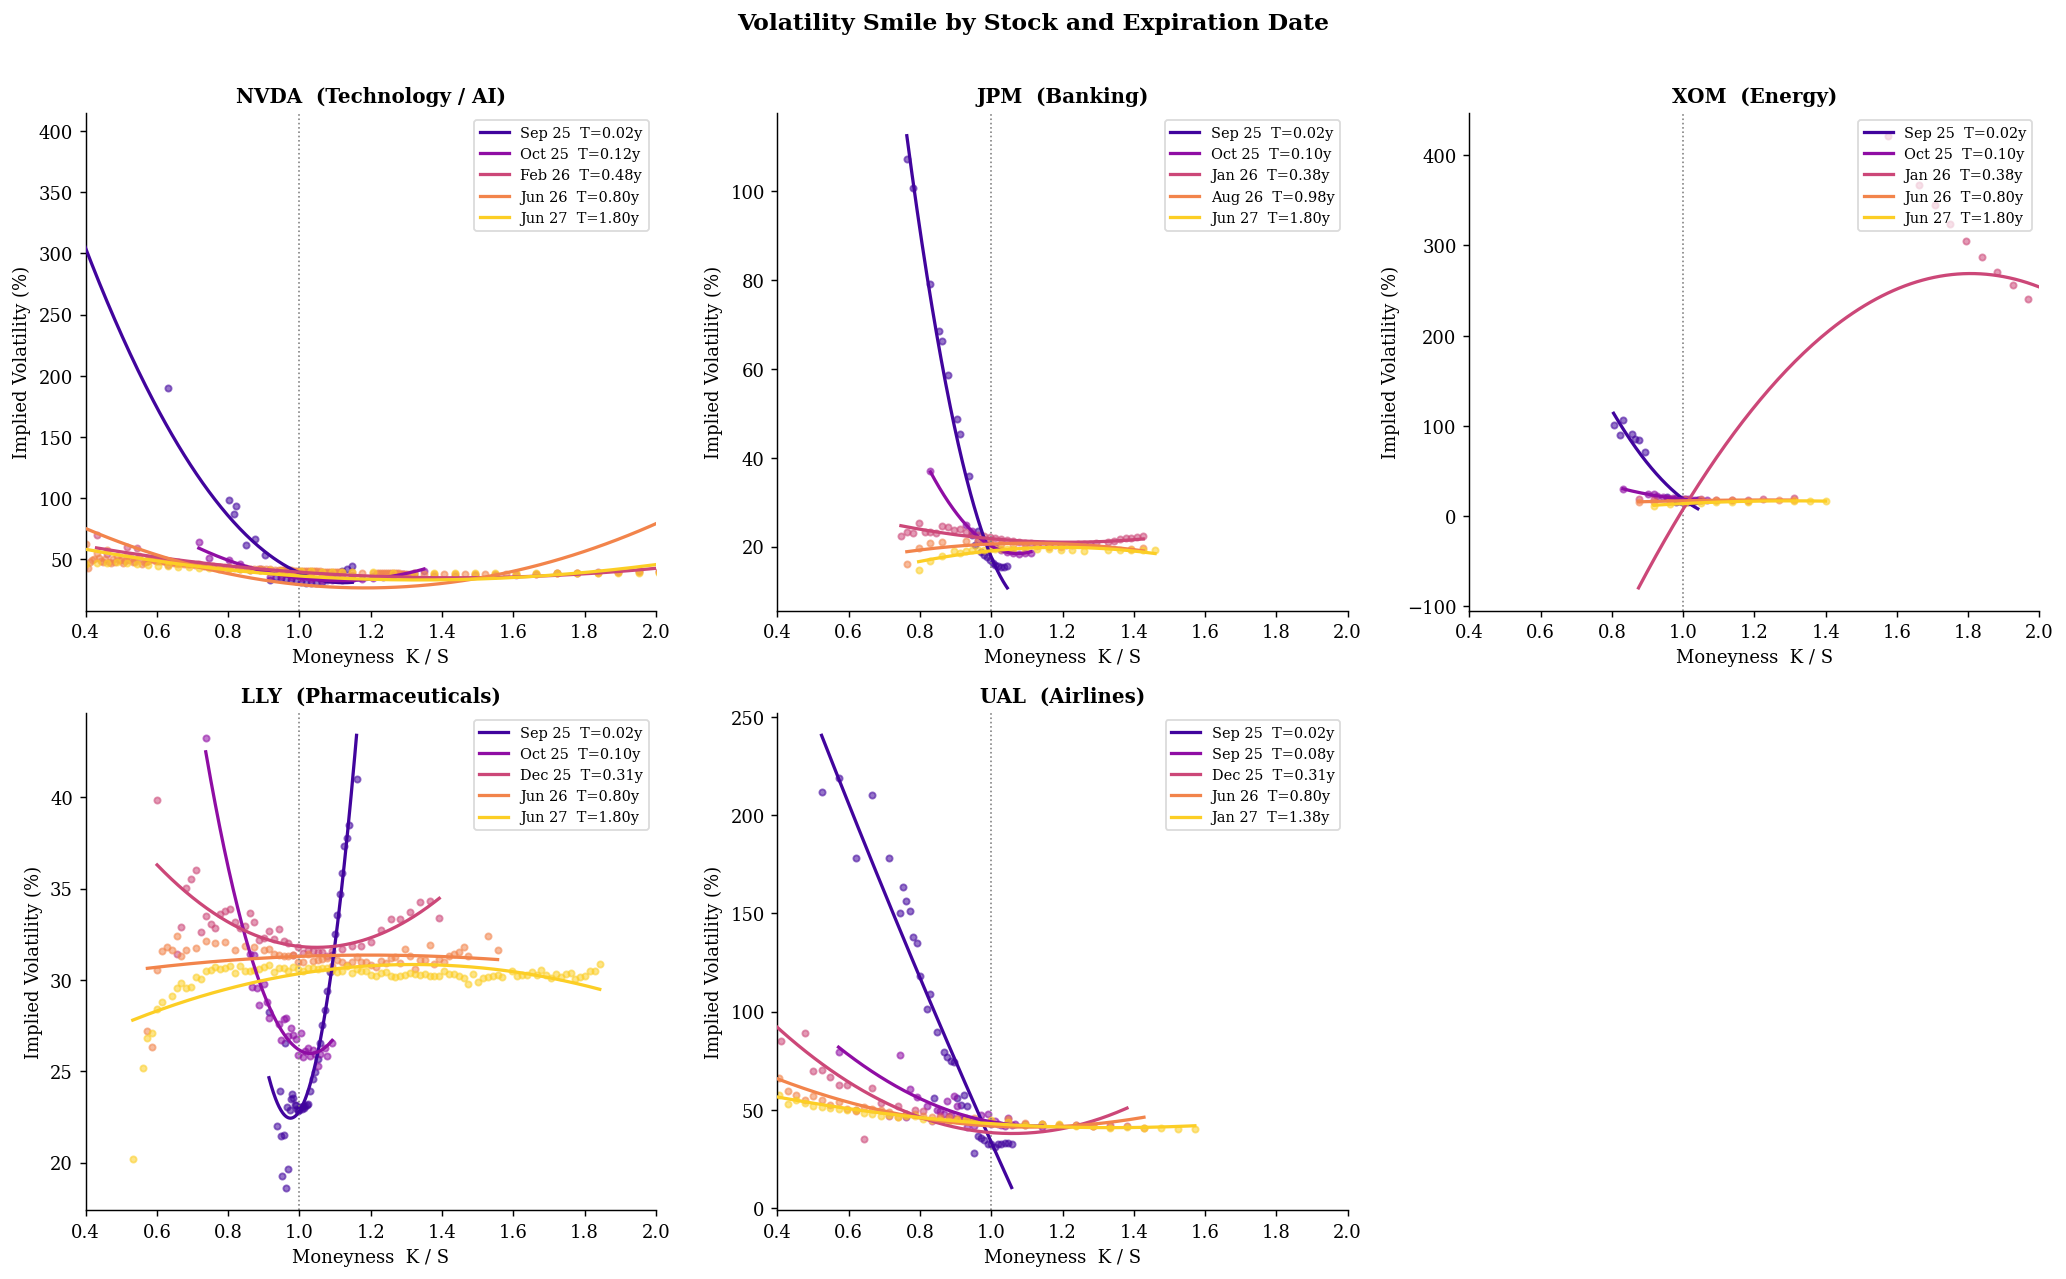
\includegraphics[width=\textwidth]{q1_smile.png}
\caption{Volatility smile for all five stocks at five expiration dates each. Points are
individual option observations; curves are quadratic polynomial fits. The dotted vertical
line marks $K/S = 1$ (at the money).}
\label{fig:smile}
\end{figure}

Every stock exhibits a negatively sloped smile at every expiration: implied volatility
is highest at low strikes and falls as the strike rises. This equity put-skew has been a
robust feature of option markets since at least \citet{Rubinstein1994}. The skew steepens
at short maturities and flattens as $T$ grows, because near-term crash risk is priced
more aggressively than long-run structural tail risk; mean-reversion in volatility
reduces the probability of sustained extreme outcomes over longer horizons.

Stock-specific patterns are as follows. \textit{NVDA}: at October 2025 ($T \approx 0.12$
years), the smile descends from roughly 55\% near $K/S = 0.75$ to 35\% at the money, a
20 percentage point drop. By June 2027 ($T = 1.80$ years), the slope narrows to about
one-fifth of its near-term value ($-7.3$ versus $-37.5$) while ATM IV rises modestly to
40\%, producing an upward-sloping term structure. \textit{XOM}: ATM IV is broadly stable
at 17--19\% at short to medium maturities but declines to 14\% at two years. The skew
slope is steep at short maturities and collapses toward zero by four months. At medium
maturities, certain expirations display a positively sloped fitted curve at high strikes,
visible in Figure~\ref{fig:smile}; this pattern is most plausibly a numerical artifact
of the quadratic fit being applied to a small number of sparse, illiquid far-out-of-the-money
call quotes rather than a genuine market-implied premium for upside \citep{Jackwerth2000}.
The near-ATM skew, which is better identified by liquid quotes, remains negative throughout.
\textit{JPM}: ATM IV traces a mild hump (20\% at one month, 22\% at four months, 19\%
at two years); the slope narrows from $-58$ to near zero across the same range, so
crash-risk pricing is almost entirely a short-horizon phenomenon. \textit{UAL}: ATM IV
is locked at approximately 44\% from one month out to 16 months, a distinctively flat
term structure reflecting persistent multi-source uncertainty. The slope does fall from
$-37$ to $-7$ over that range. \textit{LLY}: the most complete flattening of the five
stocks, with the slope moving from $-21$ at one month to essentially zero ($-0.2$) at
two years, consistent with binary event risk that resolves once clinical or regulatory
decisions are made.

\subsection{The Implied Volatility Surface}

Figures~\ref{fig:surface_heatmap} and~\ref{fig:surface_3d} display the full surface for
each stock as a heatmap and a 3D scatter, respectively.

The dominant feature in all heatmaps is the horizontal color gradient: the left (low
strike) portion is red and the right transitions to green, encoding the negative skew
simultaneously across all maturities. This gradient is most pronounced for NVDA and is
shallowest for LLY. The XOM heatmap is an exception to the otherwise clean pattern:
linear interpolation onto the regular grid propagates the influence of sparse,
illiquid far-out-of-the-money quotes, producing an elevated red region at high strikes
and medium maturities that does not reflect genuine market pricing of the upside
\citep{Jackwerth2000}. The near-ATM region of the XOM surface, which is well-identified
by liquid data, retains the expected negative skew. In the maturity dimension, most
surfaces slope slightly upward, indicating that long-horizon uncertainty is modestly
higher than near-term realized expectations, with UAL being the exception whose surface
is nearly flat across $T$. The interaction between the two dimensions, a compressed
gradient at short $T$ that diffuses at long $T$, is consistent with stochastic volatility
models in which near-term crash risk commands a premium that decays with horizon
\citep{Heston1993}.

\begin{figure}[H]
\centering
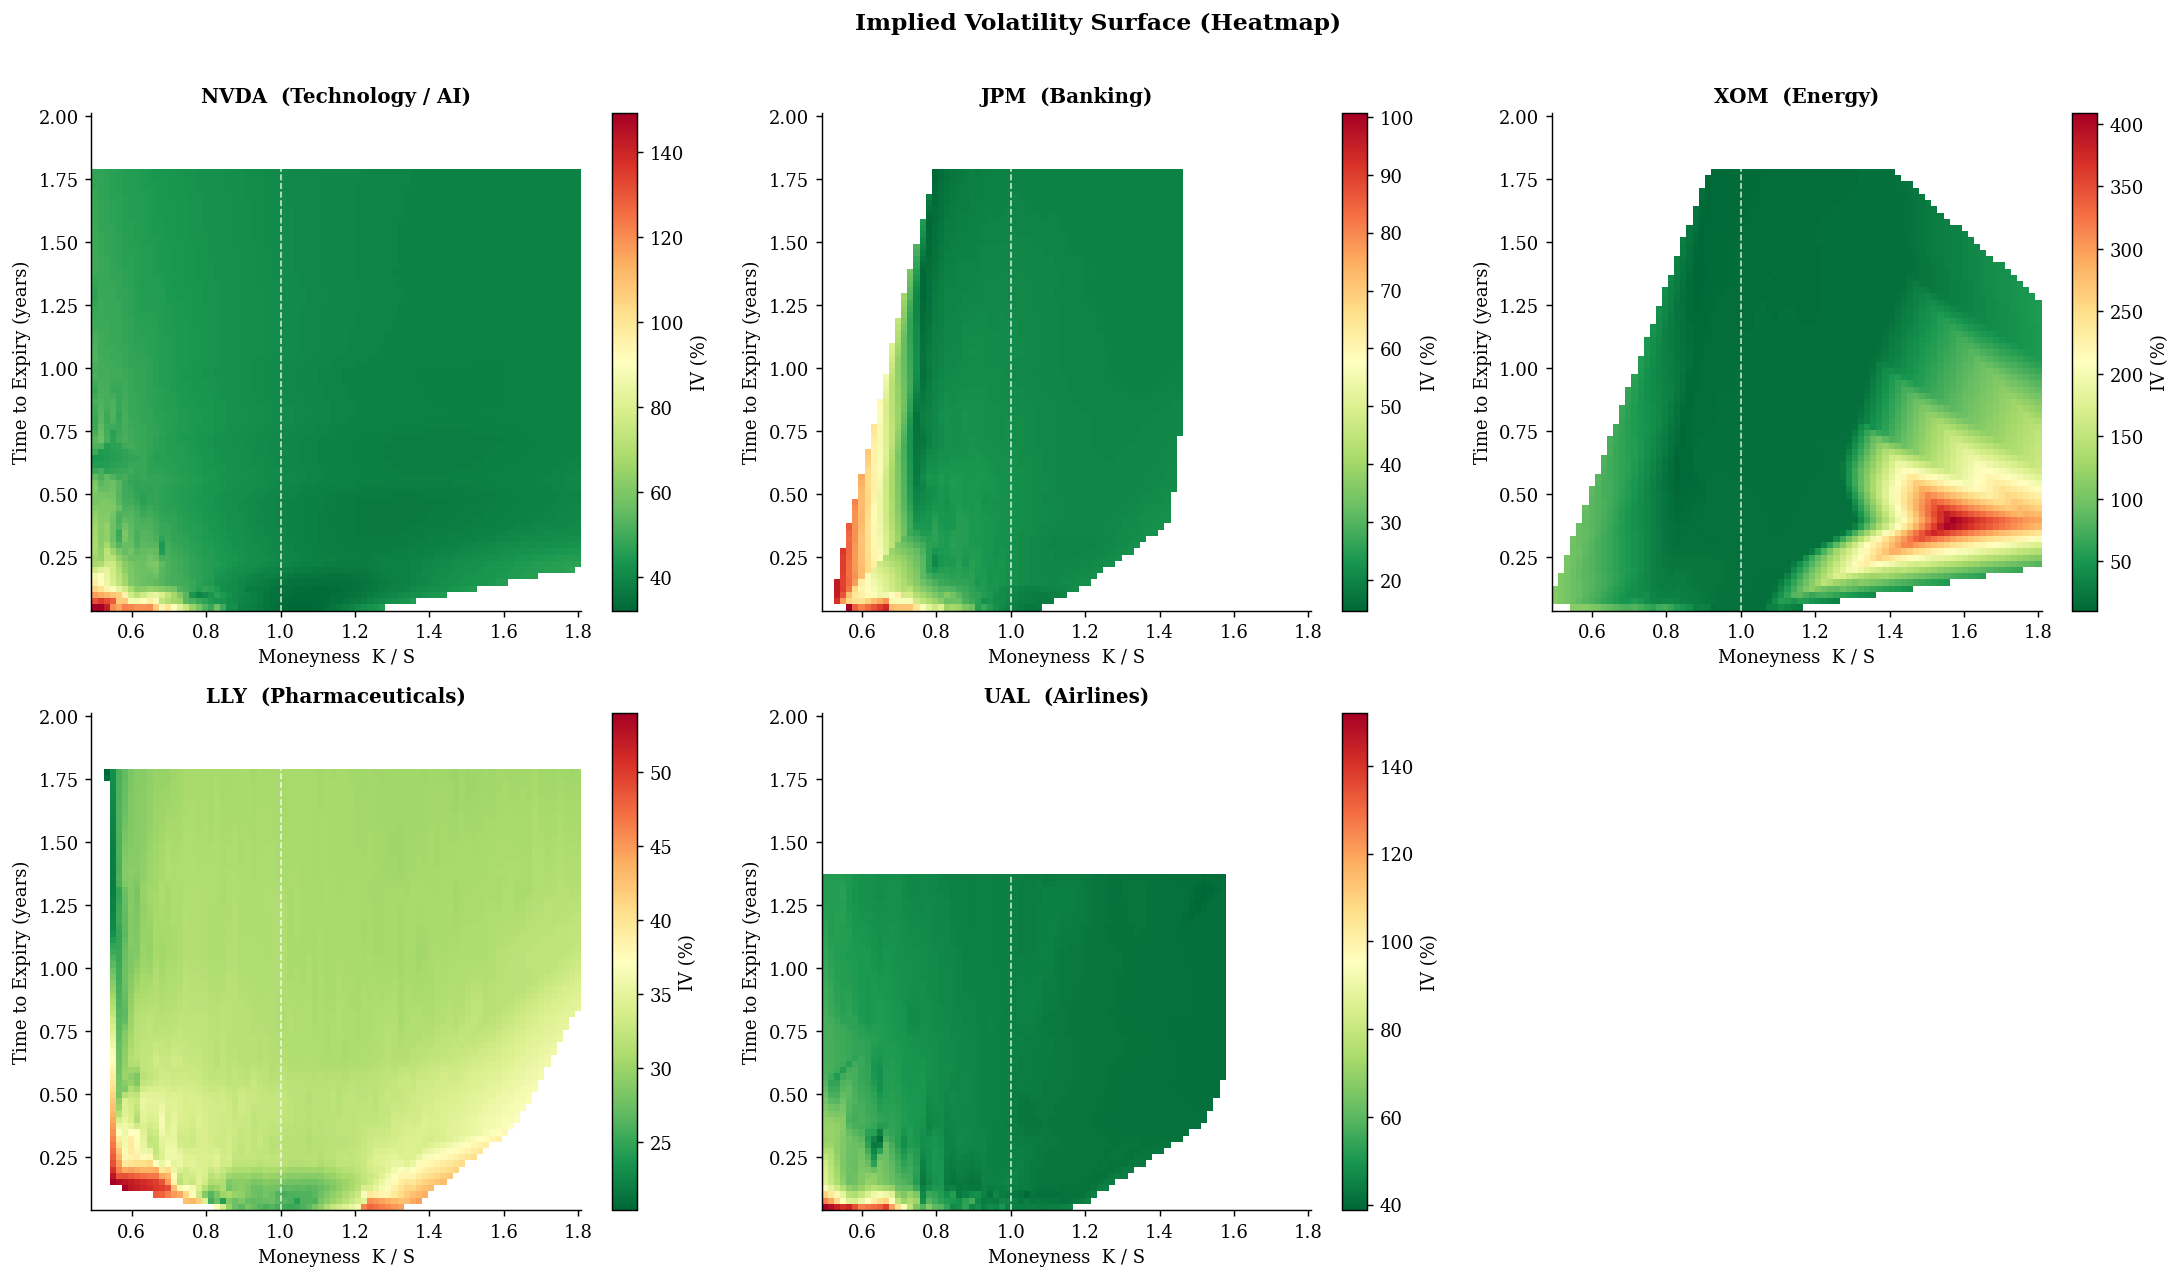
\includegraphics[width=\textwidth]{q1_surface_heatmap.png}
\caption{Implied volatility surface as a heatmap. Red: high IV; green: low IV. Values
are linearly interpolated onto a regular grid. The white dashed line marks $K/S = 1$.}
\label{fig:surface_heatmap}
\end{figure}

\begin{figure}[H]
\centering
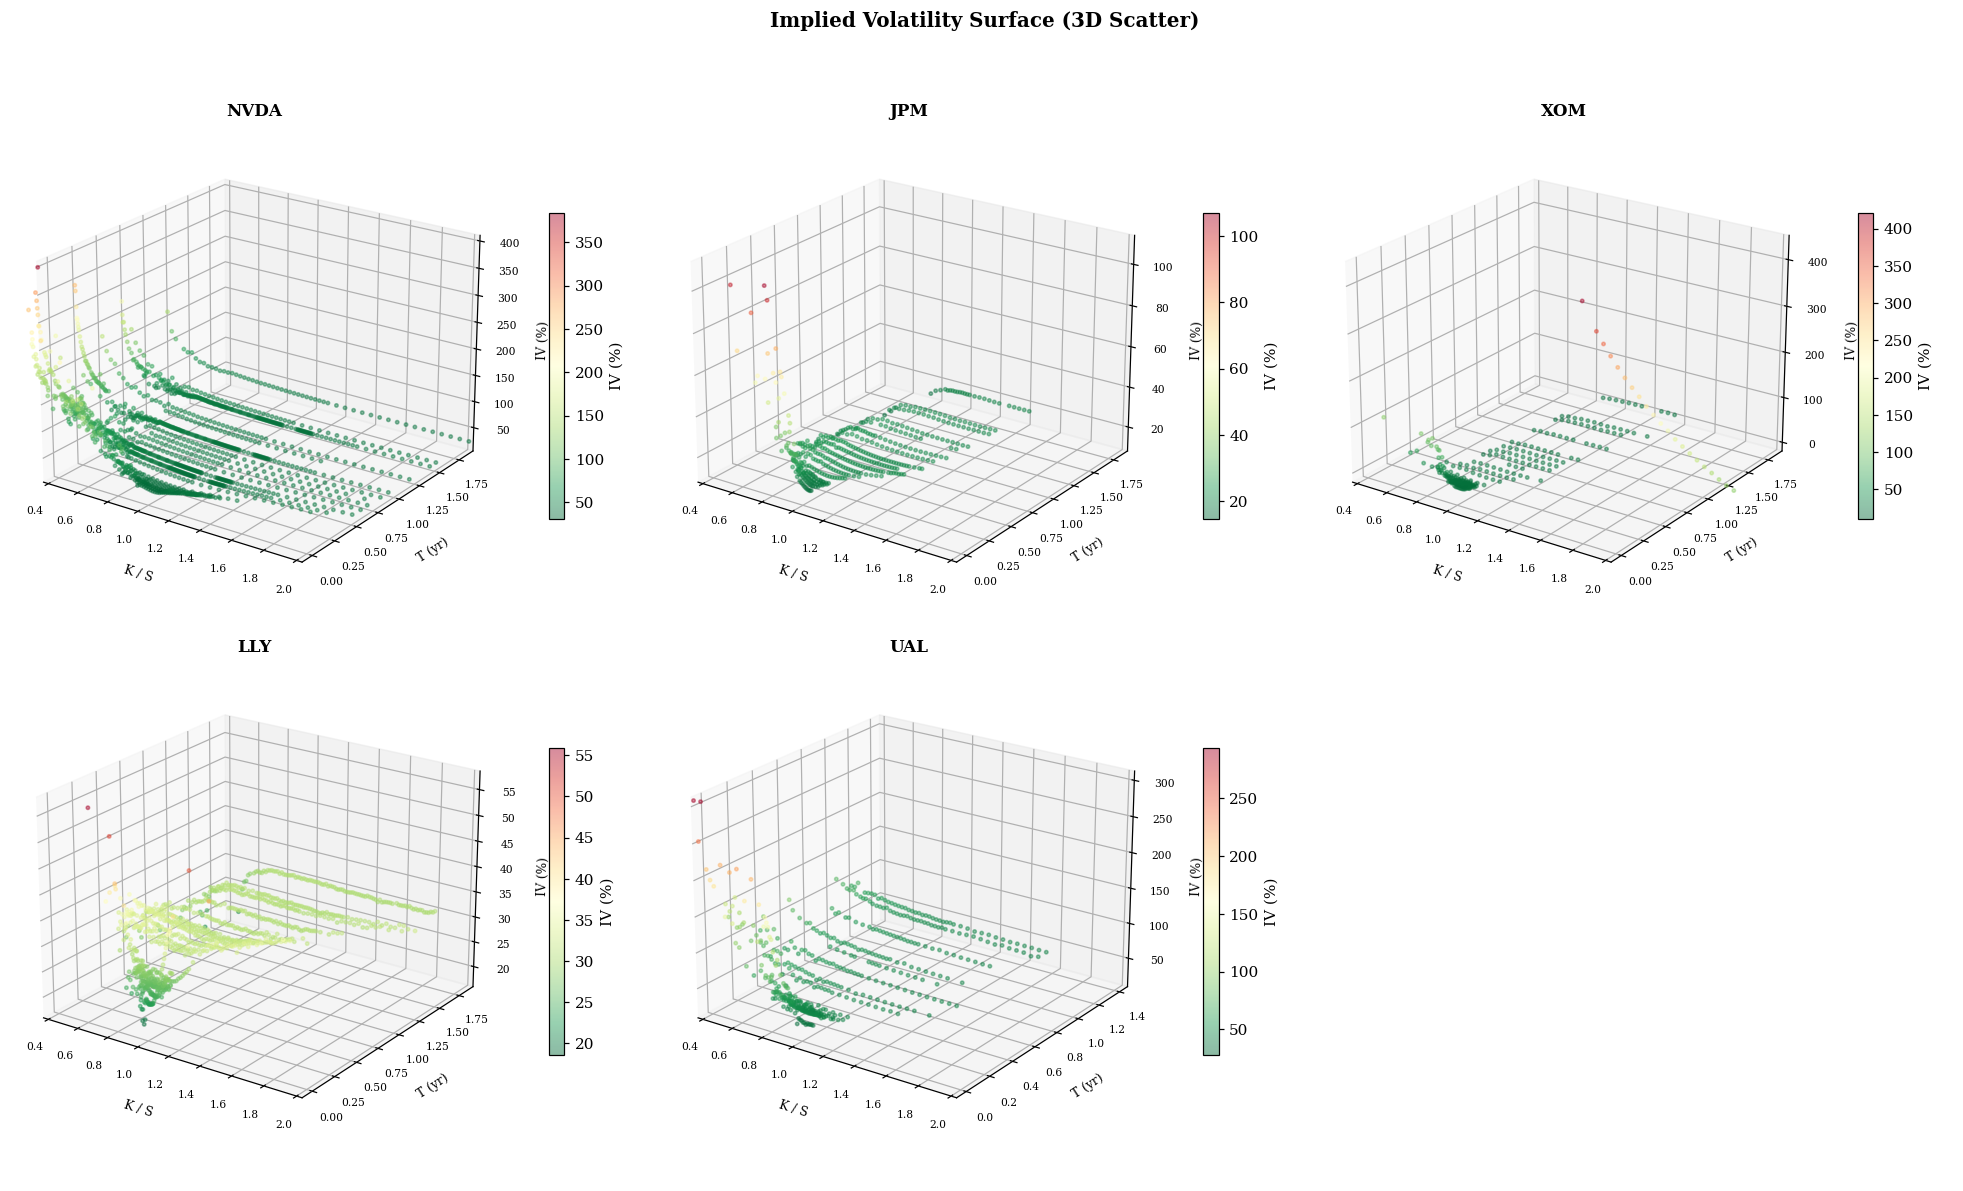
\includegraphics[width=\textwidth]{q1_surface_3d.png}
\caption{Implied volatility surface as a 3D scatter. Each point is one option; color
encodes IV level. No interpolation is applied.}
\label{fig:surface_3d}
\end{figure}

\subsection{Cross-Sectional Comparison}

\subsubsection{Methodology}

Each stock's surface is summarized by two scalars. \textbf{ATM implied volatility} is the
median IV for options with moneyness in $[0.95, 1.05]$ pooled across all maturities.
\textbf{Skew slope} is the OLS coefficient from regressing IV on moneyness for options
with $K/S \in [0.70, 1.30]$ at the expiration nearest to three months. A more negative
slope indicates a larger premium for out-of-the-money puts relative to ATM options, which
is the standard definition of the volatility skew \citep{Hull2022}.

\subsubsection{Results}
\begin{table}[H]
\centering
\caption{ATM implied volatility and skew slope at the nearest 3-month expiration.
A more negative slope indicates a steeper left skew.}
\label{tab:summary}
\begin{tabular}{llrr}
\toprule
Ticker & Sector & ATM IV (\%) & Skew Slope \\
\midrule
NVDA & Technology / AI  & 39.8 & $-23.7$ \\
JPM  & Banking           & 20.9 &  $-8.8$ \\
XOM  & Energy            & 18.1 & $-21.8$ \\
LLY  & Pharmaceuticals   & 26.9 &  $-4.7$ \\
UAL  & Airlines          & 44.0 & $-14.3$ \\
\bottomrule
\end{tabular}
\end{table}

\begin{figure}[H]
\centering
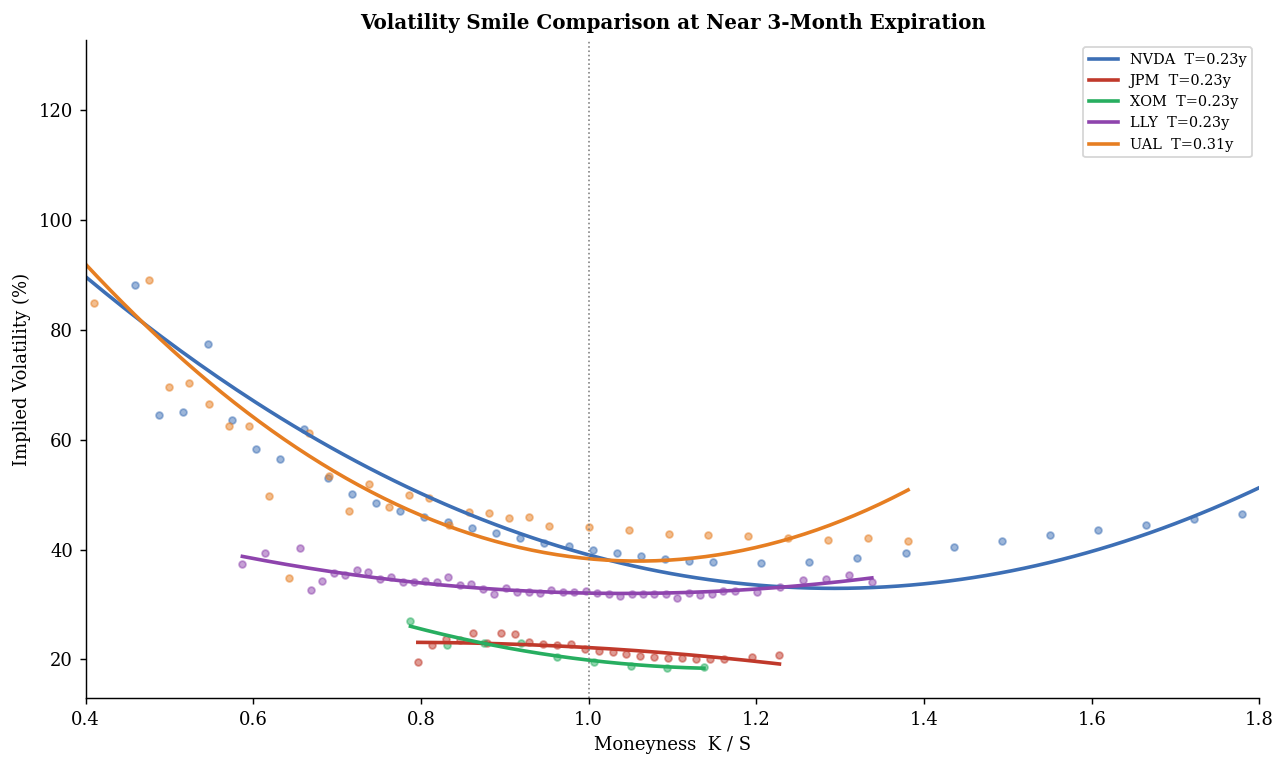
\includegraphics[width=0.75\textwidth]{q1_smile_overlay.png}
\caption{Smile overlay at the nearest 3-month expiration for direct cross-sectional
comparison.}
\label{fig:overlay}
\end{figure}

\begin{figure}[H]
\centering
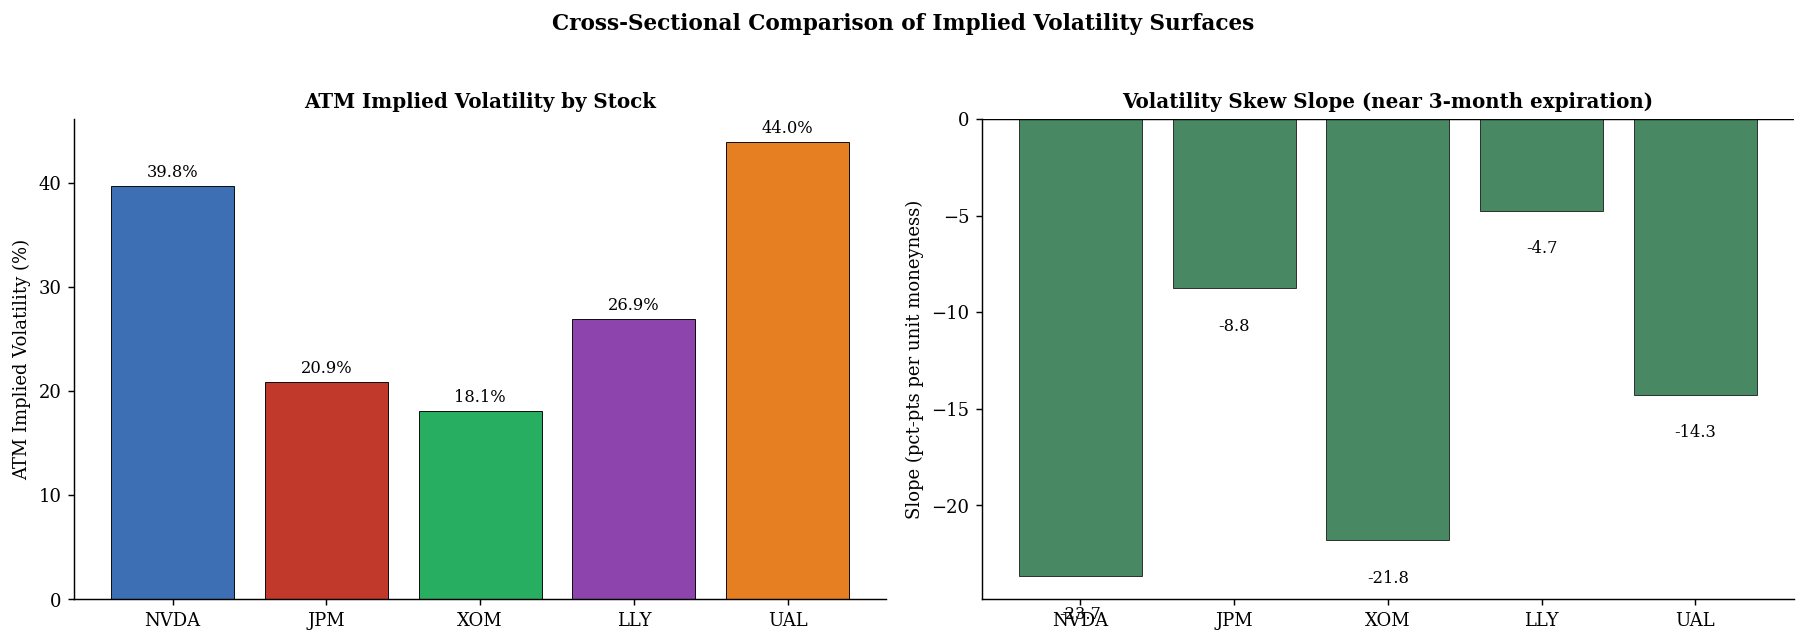
\includegraphics[width=\textwidth]{q1_comparison.png}
\caption{ATM implied volatility (left) and skew slope (right) for all five stocks.}
\label{fig:comparison}
\end{figure}

Table~\ref{tab:summary} and Figures~\ref{fig:overlay}--\ref{fig:comparison} present the
summary statistics and cross-sectional comparisons.

\subsubsection{Interpretation}

\textbf{UAL leads on ATM IV (44.0\%).} Airlines combine high fixed costs, thin margins,
and exposure to uncontrollable inputs (fuel, demand cycles, regulation), producing equity
return distributions with fat tails in both directions. The market prices this as
persistently elevated ATM volatility.

\textbf{NVDA second on ATM IV (39.8\%) and steepest skew ($-23.7$).} NVIDIA's valuation
was heavily linked to AI infrastructure investment through 2023--2025, making the stock
sensitive to sentiment shifts in GPU demand. A stock that has appreciated rapidly on a
speculative theme carries asymmetric downside risk: the gain can be quickly reversed
without an equivalent probability of a further gain. Investors accumulated put protection
aggressively, bidding up the left wing and producing a steep skew despite the absence of
the regulatory or commodity risk present in other sectors.

\textbf{XOM second steepest skew ($-21.8$) despite the lowest ATM IV (18.1\%).} The
skew slope reported in Table~\ref{tab:summary} is estimated over the liquid near-ATM
range $K/S \in [0.70, 1.30]$, where XOM quotes are well identified. Energy equity faces
a specific directional risk: commodity price collapse. Historical oil price crashes have
been severe and rapid (1986, 1998, 2008, 2014, 2020), and this asymmetric left-tail
history is reflected in energy option pricing as a steep near-ATM skew \citep{Doran2008}.
The contrast with UAL illustrates that IV level and skew slope measure different things:
UAL's uncertainty is multidirectional and elevates the ATM level broadly, while XOM's
dominant risk is directional and concentrates the premium in the left wing.

\textbf{LLY shallowest skew ($-4.7$).} Pharmaceutical equity faces two-sided binary
event risk from clinical and regulatory outcomes. Because the downside (trial failure) is
not systematically more probable or more severe than the upside (approval), the smile is
close to symmetric. LLY's ATM IV of 26.9\% exceeds XOM's precisely because uncertainty
is elevated but not directionally biased.

\textbf{JPM: bank vs.\ technology vs.\ airline.} JPM's skew of $-8.8$ is the second
shallowest despite banking's well-documented systemic risk. The Federal Reserve
stress-testing framework, Basel III capital requirements, and FDIC deposit guarantees
collectively bound the probability of the most catastrophic left-tail outcomes for large
US banks. NVDA's AI rerating risk and UAL's operating leverage carry no equivalent
institutional backstop, which is why both generate steeper skews than a bank with
balance-sheet exposure to the entire economy.

\textbf{Black--Scholes implication.} The non-flat surface is direct evidence of model
misspecification: real return distributions exhibit negative skewness and excess kurtosis
relative to the log-normal \citep{Rubinstein1994}. Stochastic volatility models, such as
\citet{Heston1993}, address this by allowing instantaneous variance to follow its own
mean-reverting process, which generates the maturity-dependent negative skew that
Black--Scholes cannot produce.

% ============================================================
\section{Option Pricing: Black-Scholes, Monte Carlo, and Binomial Trees}
% ============================================================

In this section, we price the same European call option using three different 
approaches: Black-Scholes (closed-form), Monte Carlo simulation, and a binomial lattice model. 
The chosen stock for the European call option is Eli Lilly and Company (LLY).

We use the following information for the pricing:
- On April 10th, 2026, LLY closed at $939.47 per share (CITE). 
- As of April 9th, 2026, the risk-free rate for U.S. Treasury Securities at 6-Month Constant Maturity is 3.71\% (CITE).
- The time to expiry is 6 months.
- For an at-the-money European call option, the strike price is equal to the stock price, $939.47.
- The at-the-money implied volatility for LLY, calculated in Section 1, is 26.90\%. 

\subsubsection{Black-Scholes}

In this section, we price the European call option using the Black-Scholes formula.
The Black-Scholes formula for a European call option is:

$$C = S\,N(d_1) - K e^{-rT} N(d_2), \qquad
d_1 = \frac{\ln(S/K) + (r + \sigma^2/2)\,T}{\sigma\sqrt{T}}, \quad
d_2 = d_1 - \sigma\sqrt{T},
$$
where $S$ is the stock price, $K$ is the strike price, $T$ is the time to expiry, $r$ is the risk-free rate, and $\sigma$ is the implied volatility.
$N(\cdot)$ is the standard normal cumulative distribution function (CDF).

[TODO: expand?]

The Black-Scholes price of the LLY call option is \$79.50.
We use this price as the benchmark for the Monte Carlo and binomial lattice pricing.

[TODO: interpret?]

\subsubsection{Monte Carlo}



\subsubsection{Binomial Lattice}

% ============================================================
\section{Pricing Exotic Options}
% ============================================================

Using Monte Carlos, we can price \textit{any} derivative whose payoff can be simulated, which wasn't possible using geometric Brownian motion. In particular, path-dependent options for which no closed-form solution exists can also be priced using Monte Carlo. We
price two such exotic options on LLY using the same parameters as Section~2: $S_0 =
\$939.47$, $K = \$939.47$ (at the money), $T = 0.5$ years, $r = 3.71\%$, $\sigma =
26.90\%$. Full daily price paths are simulated via the Euler--Maruyama scheme with
$n = 126$ steps ($\Delta t = T/n$). The number of paths $N$ is chosen so that the
Monte Carlo standard error is below \$0.9395 (0.1\% of $S_0$); we use $N = 1{,}000{,}000$
throughout and verify the criterion is met for both options.

\subsection{Arithmetic Asian Call}

The \textbf{arithmetic Asian call} replaces the terminal stock price $S_T$ with the
time-average over the life of the option:
\begin{equation}
    \text{Payoff} = \max(\bar{S} - K,\; 0), \qquad
    \bar{S} = \frac{1}{n} \sum_{i=1}^{n} S_{t_i}.
    \label{eq:asian}
\end{equation}
No closed-form solution exists for this payoff under geometric Brownian motion. The simulation
tracks the running sum of prices at each of the 126 daily steps and divides by $n$ at
expiry to obtain $\bar{S}$ without storing full path matrices. 

\begin{table}[H]
\centering
\caption{Arithmetic Asian call results ($N = 1{,}000{,}000$ paths).}
\label{tab:asian}
\begin{tabular}{lr}
\toprule
Metric & Value \\
\midrule
MC price                & \$45.37 \\
Simulation Time         & 1.18 s \\
Standard error (SE)     & \$0.07 \\
SE criterion met?       & Yes (\$0.07 $<$ \$0.94) \\
95\% confidence interval & [\$45.24,\ \$45.51] \\
Black--Scholes benchmark & \$79.50 \\
Asian vs.\ vanilla      & $-$\$34.12 ($-$42.9\%) \\
\bottomrule
\end{tabular}
\end{table}

The Asian call costs \$45.37, roughly 43\% less than the vanilla European call at
\$79.50. Averaging dampens the effective volatility of the payoff: extreme terminal
prices, whether very high or very low, are pulled toward the path mean, so the
distribution of $\bar{S}$ has lower variance than that of $S_T$. By having lower volatility, the option is less risky, and thus, has a lower option premium. 

\subsection{Floating-Strike Lookback Call}

The \textbf{floating-strike lookback call} sets the strike retroactively to the minimum
price reached over the life of the option, giving the holder perfect hindsight on entry:
\begin{equation}
    \text{Payoff} = S_T - \min_{0 \le t \le T} S_t.
    \label{eq:lookback}
\end{equation}
The payoff is \textit{always non-negative} by construction: $S_T \ge \min_{t} S_t$
holds on every path. 
\begin{table}[H]
\centering
\caption{Floating-strike lookback call results ($N = 1{,}000{,}000$ paths).}
\label{tab:lookback}
\begin{tabular}{lr}
\toprule
Metric & Value \\
\midrule
MC price                & \$134.33 \\
Standard error (SE)     & \$0.12 \\
SE criterion met?       & Yes (\$0.12 $<$ \$0.94) \\
95\% confidence interval & [\$134.09,\ \$134.57] \\
Black--Scholes benchmark & \$79.50 \\
Lookback vs.\ vanilla   & $+$\$54.83 ($+$69.0\%) \\
\bottomrule
\end{tabular}
\end{table}

The lookback option costs \$134.33, a 69\% premium over the vanilla call. Two effects
drive this: \\

First, the payoff can never be zero: on every single path the holder profits
by at least the difference between $S_T$ and the path minimum, whereas a vanilla call
expires worthless whenever $S_T < K$. \\

Second, the effective strike depends on the path because it is retroactively determined after the fact. On a path that dips to \$800 before recovering to \$950, the
lookback pays \$150 while the ATM vanilla pays only \$10.53. The real-world motivation for paying this premium is perfect downside protection combined with full upside participation: an investor who fears missing the optimal entry point but still wants equity exposure would find the lookback compelling, albeit expensive.

\subsection{Comparison}

Table~\ref{tab:exotic_comparison} and Figure~\ref{fig:q3_comparison} summarize all three
options. The pricing hierarchy---Asian $<$ Vanilla $<$ Lookback---reflects the
information available to each payoff function at expiry. The vanilla call uses only the
terminal price; the Asian call uses the average, which is less extreme; the lookback call
uses both the terminal price and the worst-case entry, the most favorable possible
information set.

\begin{table}[H]
\centering
\caption{Summary comparison: vanilla European call (Black--Scholes) vs.\ two exotic calls (Monte Carlo, $N = 1{,}000{,}000$).}
\label{tab:exotic_comparison}
\begin{tabular}{llrrl}
\toprule
Option & Method & Price (\$) & SE (\$) & Payoff \\
\midrule
Vanilla European  & Black--Scholes   & 79.50  & --- & $\max(S_T - K,\;0)$ \\
Arithmetic Asian  & Monte Carlo      & 45.37  & 0.07 & $\max(\bar{S} - K,\;0)$ \\
Floating Lookback & Monte Carlo      & 134.33 & 0.12 & $S_T - \min_t S_t$ \\
\bottomrule
\end{tabular}
\end{table}

The Asian call provides the least ``insurance'': the averaging means it pays out less
even when markets move favourably, making it the cheapest but also the least protective
instrument. The lookback provides the most insurance: it guarantees the holder the
best possible entry price in hindsight, making it the most expensive. The vanilla call
sits in between, paying out only if the terminal price exceeds the fixed strike.

\begin{figure}[H]
\centering
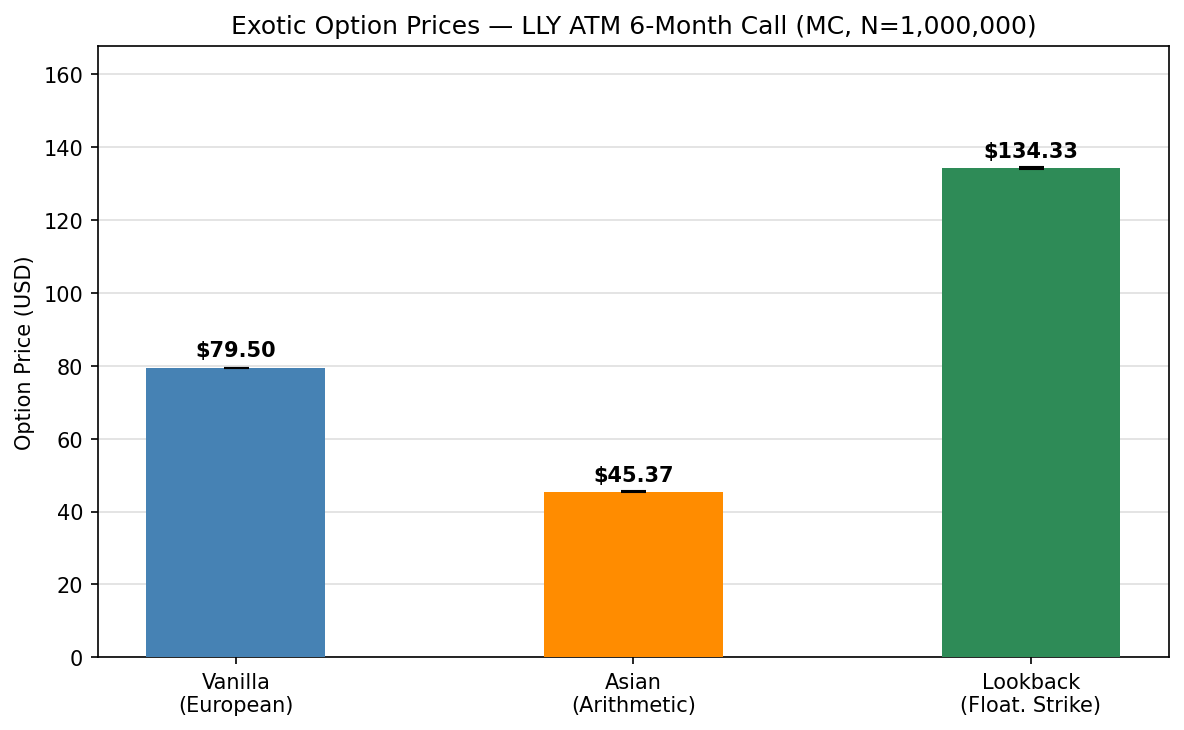
\includegraphics[width=0.80\textwidth]{q3_comparison.png}
\caption{Monte Carlo prices for the three LLY 6-month call options. Error bars show
95\% confidence intervals ($\pm 1.96 \times \text{SE}$). The vanilla price is exact
(Black--Scholes); MC uncertainty bars for Asian and lookback options are narrower than
the bar width at this scale.}
\label{fig:q3_comparison}
\end{figure}

% ============================================================
\section{The CIR Model and Bond Pricing}
% ============================================================

% ============================================================
\section{Hedging a Bank's Interest Rate Risk}
% ============================================================

% ============================================================
\section{AI Disclosure}
% ============================================================

Large language models were used for task explanation, code debugging, and \LaTeX{}
formatting. All analysis, interpretation, and written discussion were produced and
verified by the group.

% ============================================================
\bibliographystyle{plainnat}
\begin{thebibliography}{99}

\bibitem[Black and Scholes(1973)]{BlackScholes1973}
Black, F.\ and Scholes, M.\ (1973).
The pricing of options and corporate liabilities.
\textit{Journal of Political Economy}, 81(3), 637--654.

\bibitem[Brent(1973)]{Brent1973}
Brent, R.\ P.\ (1973).
\textit{Algorithms for Minimization without Derivatives}.
Prentice-Hall, Englewood Cliffs, NJ. Chapter~4.

\bibitem[Board of Governors(2025)]{FRED_DGS1}
Board of Governors of the Federal Reserve System (US) (2025).
1-Year Treasury Constant Maturity Rate [DGS1].
Federal Reserve Bank of St.\ Louis FRED database.
Retrieved from \url{https://fred.stlouisfed.org/series/DGS1}, August 29, 2025.

\bibitem[Doran and Ronn(2008)]{Doran2008}
Doran, J.\ S.\ and Ronn, E.\ I.\ (2008).
Computing the market price of volatility risk in the energy commodity markets.
\textit{Journal of Banking and Finance}, 32(12), 2541--2552.

\bibitem[Heston(1993)]{Heston1993}
Heston, S.\ L.\ (1993).
A closed-form solution for options with stochastic volatility with applications to bond
and currency options.
\textit{Review of Financial Studies}, 6(2), 327--343.

\bibitem[Hull(2022)]{Hull2022}
Hull, J.\ C.\ (2022).
\textit{Options, Futures, and Other Derivatives}, 11th ed.
Pearson, New York.

\bibitem[Jackwerth(2000)]{Jackwerth2000}
Jackwerth, J.\ C.\ (2000).
Recovering risk aversion from option prices and realized returns.
\textit{Review of Financial Studies}, 13(2), 433--451.

\bibitem[Rubinstein(1994)]{Rubinstein1994}
Rubinstein, M.\ (1994).
Implied binomial trees.
\textit{Journal of Finance}, 49(3), 771--818.

\end{thebibliography}

\end{document}